% 8 points P_i = rot^i(6,0), Q_i = rot^i(1,2): no three collinear, no 5 in convex position (all 56 subsets checked).
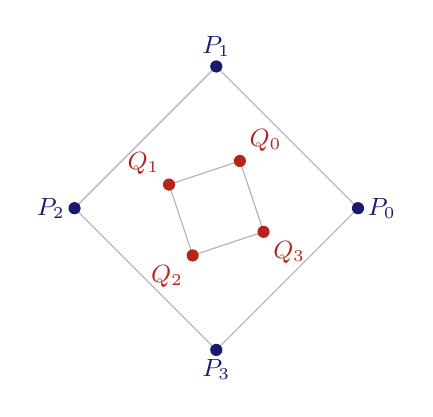
\begin{tikzpicture}[font=\small]
\draw[black!30] (1.8000,0.0000) -- (0.0000,1.8000) -- (-1.8000,0.0000) -- (0.0000,-1.8000) -- cycle;
\draw[black!30] (0.3000,0.6000) -- (-0.6000,0.3000) -- (-0.3000,-0.6000) -- (0.6000,-0.3000) -- cycle;
\fill[MidnightBlue] (1.8000,0.0000) circle (2.2pt) node[right] {$P_0$};
\fill[MidnightBlue] (0.0000,1.8000) circle (2.2pt) node[above] {$P_1$};
\fill[MidnightBlue] (-1.8000,0.0000) circle (2.2pt) node[left] {$P_2$};
\fill[MidnightBlue] (0.0000,-1.8000) circle (2.2pt) node[below] {$P_3$};
\fill[BrickRed] (0.3000,0.6000) circle (2.2pt) node[above right] {$Q_0$};
\fill[BrickRed] (-0.6000,0.3000) circle (2.2pt) node[above left] {$Q_1$};
\fill[BrickRed] (-0.3000,-0.6000) circle (2.2pt) node[below left] {$Q_2$};
\fill[BrickRed] (0.6000,-0.3000) circle (2.2pt) node[below right] {$Q_3$};
\end{tikzpicture}
